\documentclass{article}
\usepackage{graphicx}
\usepackage{booktabs}
\usepackage{float}
\usepackage{geometry}
\geometry{margin=1in}
\begin{document}

\section*{Análisis RAG}
\subsection*{Moda de categorías}
\begin{table}[H]
\centering
\begin{tabular}{ll}
\toprule
\textbf{Métrica} & \textbf{Moda (frecuencia)} \\
\midrule
Cobertura & buena (2) \\
Precisión & alta (3) \\
Alucinacion & False (3) \\
\bottomrule\n\end{tabular}\n\caption{Moda por categoría en las métricas RAG}\n\end{table}\n\subsection*{Media y desviación típica de los chunks}
\begin{table}[H]
\centering
\begin{tabular}{lll}
\toprule
\textbf{Campo} & \textbf{Media} & \textbf{Desviación típica} \\
\midrule
chunks\_rag & 6.00 & 5.48 \\
chunks\_reranking & 9.60 & 8.96 \\
chunks\_relevantes & 9.60 & 8.96 \\
chunks\_omitidos & 3.60 & 3.78 \\
\bottomrule\n\end{tabular}\n\caption{Media y desviación típica de chunks}\n\end{table}\n
\subsection*{Gráfico de frecuencias}
\begin{figure}[H]
\centering
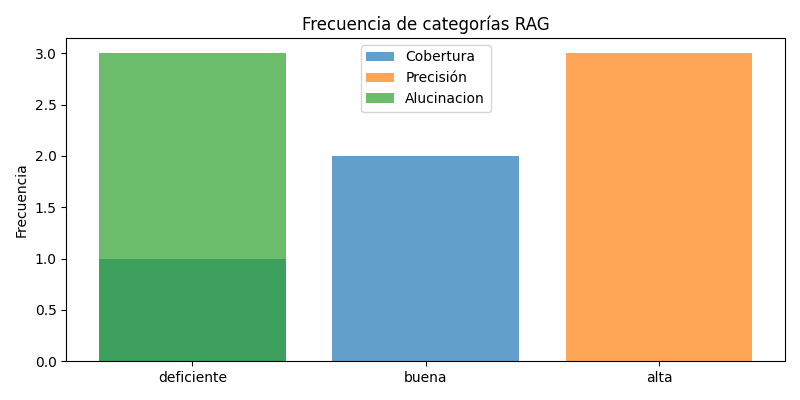
\includegraphics[width=0.8\textwidth]{../graficos/frecuencias_rag.png}
\caption{Frecuencia de categorías en las métricas RAG}
\end{figure}
\end{document}